% ----------------------------------------------------------------------
%                   LATEX TEMPLATE FOR PhD THESIS
% ----------------------------------------------------------------------

% based on Harish Bhanderi's PhD/MPhil template, then Uni Cambridge
% http://www-h.eng.cam.ac.uk/help/tpl/textprocessing/ThesisStyle/
% corrected and extended in 2007 by Jakob Suckale, then MPI-CBG PhD programme
% and made available through OpenWetWare.org - the free biology wiki


%: Style file for Latex
% Most style definitions are in the external file PhDthesisPSnPDF.
% In this template package, it can be found in ./Latex/Classes/
\documentclass[twoside,11pt]{Latex/Classes/PhDthesisPSnPDF}

%: Macro file for Latex
% Macros help you summarise frequently repeated Latex commands.
% Here, they are placed in an external file /Latex/Macros/MacroFile1.tex
% An macro that you may use frequently is the figuremacro (see introduction.tex)
\include{Latex/Macros/macros}

\DeclareMathAlphabet{\mathcal}{OMS}{cmsy}{m}{n}

%glossary ralated code
\usepackage[toc]{glossaries}
\renewcommand*{\glossaryentrynumbers}[1]{}
%\setlength{\glsdescwidth}{0.8\linewidth}
\makeglossaries

\glossarystyle{list}
\renewcommand*{\glsgroupskip}{}

\addbibresource[]{bibliography.bib}


% this file is called up by thesis.tex
% content in this file will be fed into the main document

% 1 = Entry name, e.g. abbreviation; 2 = Explanation
% You can place all explanations in this separate file or declare them in the middle of the text. Either way they will be collected in the glossary.

% required to print nomenclature name to page header
\newacronym{SLAM}{SLAM}{Simultaneous Localization And Mapping}
\newacronym{LRF}{LRF}{Laser Range Finder}
\newacronym{aLRF}{aLRF}{actuated Laser Range Finder}
\newacronym{NBV}{NBV}{Next Best Viewpoint}
\newacronym{FoV}{FoV}{Field of View}
\newacronym{ToF}{ToF}{Time of Flight}
%\newacronym{NNS}{NNS}{Nearest Neighbor Search}
\newacronym{EGI}{EGI}{Extended Gaussian Image}
%\newacronym{PCA}{PCA}{Principal Component Analysis}
\newacronym{MSE}{MSE}{Mean Square Error}
\newacronym{ICP}{ICP}{Iterative Closest Point}
\newacronym{NDT}{NDT}{Normal Distributions Transform}
\newacronym{3D-NDT}{3D-NDT}{Three-Dimensional Normal Distributions Transform}
\newacronym{MUMC}{MUMC}{Minimum Uncertainty Maximum Consensus}
\newacronym{IMU}{IMU}{Inertial Measurement Units}
\newacronym{GNSS}{GNSS}{Global Navigation Satellite Systems}
%\newacronym{EKF}{EKF}{Extended Kalman Filter}
%\newacronym{MLS}{MLS}{Multi-Level Surface}
\newacronym{PDF}{PDF}{Probability Density Functions}
%\newacronym{MLE}{MLE}{Maximum-Likelihood Estimation}
%\newacronym{P2D}{P2D}{Point-to-Distribution}
%\newacronym{FPFH}{FPFH}{Fast Point Feature Histograms}
%\newacronym{DIFT}{DIFT}{Depth-interpolated Image FeaTures}
\newacronym{RANSAC}{RANSAC}{RANdom SAmple Consensus}
\newacronym{SVM}{SVM}{Support Vector Machine}
\newacronym{PTU}{PTU}{Pan-Tilt Unit}
\newacronym{FILO}{FILO}{First-In-Last-Out}


%: ----------------------------------------------------------------------
%:                  TITLE PAGE: name, degree,..
% ----------------------------------------------------------------------
\ifpdf
    \pdfinfo { /Title  (PhD Thesis)
               /Creator (TeX)
               /Producer (pdfTeX)
               /Author (Benjamin Adler adler@informatik.uni-hamburg.de)
               /CreationDate (D:20140120)  %format D:YYYYMMDDhhmmss
               /ModDate (D:20140502)
               /Subject (robotics)
               /Keywords (Autonomous Robotics, Exploration, Mapping, SLAM) }
    \pdfcatalog { /PageMode (/UseOutlines)
                  /OpenAction (fitbh)  }
\fi

% ----------------------------------------------------------------------

% turn of those nasty overfull and underfull hboxes
\hbadness=10000
\hfuzz=50pt
%: --------------------------------------------------------------
%:                  FRONT MATTER: dedications, abstract,..
% --------------------------------------------------------------
%\makeglossaries
\begin{document}
% sets line spacing
\renewcommand\baselinestretch{1.0}
\baselineskip=14pt plus1pt

%: ----------------------- generate cover page ------------------------

\maketitle  % command to print the title page with above variables

%: ----------------------- tie in front matter ------------------------
%\frontmatter
\reviewers
%\include{0_frontmatter/dedication}
%\phantomsection
\chapter*{Change list}
\markboth{\MakeUppercase{Change list}}{}
\addcontentsline{toc}{chapter}{Change list}

\begin{itemize}
 \item Figure 3.2(b), the horizontal field of view has been corrected to 360 degrees.
 \item Algorithm 4.4, line 1, duplicate of Q <-- emptyset.
\end{itemize}
% Thesis Acknowledgements ------------------------------------------------
\phantomsection
\chapter*{Acknowledgements}
\markboth{\MakeUppercase{Acknowledgements}}{}
\addcontentsline{toc}{chapter}{Acknowledgements}

\if0
Doing a PhD was a long and exciting journey, which would not be possible without the help and support of many people. First of all I am most grateful to my supervisor Prof. Dr. Jianwei Zhang for giving me the opportunity to pursue a PhD at the University of Hamburg and providing me such a good and liberal academic environment. 

Next, I would like to extend my thanks to my daily supervisor and good friend Prof. Dr. Houxiang Zhang, whose support was always there for both technical and personal problems, not only in the first two years of my study when he was in Hamburg, but also for the second two years after he moved to {\AA}lesund. His constructive criticism helped focus my ideas and his constant encouragement kept me going in spite of many stumbling blocks on the road.    

Writing a dissertation is no easy task, but the same can be said of reviewing it. I would like to thank all the people who helped by reviewing parts of this work, especially my external reviewers --- Prof. Dr. Reinhard Koch and Dr. Peer Stelldinger. 

%I have to say, without your encouragement, I was almost going to drop when the traffic accident came to me while I had been ill for a long time. 

All the members of our TAMS group are greatly acknowledged, the time spent with you was wonderful. I own a great deal to Tatjana (Lu) Tetsis, thank you for helping me so much during the past time. My sincere thanks also go to Benjamin Adler for always being excited about my problems and ideas, always sharing his ideas with me, and the engaging discussions we had during and after work. 

I am grateful to my former colleagues from NuBot, Huimin Lu, Xiangke Wang, and Shaowu Yang are especially acknowledged, thanks a lot for valuable comments and suggestions on my conference and journal papers, as well as this dissertation. 

%I am thankful to all the people who helped by reviewing this work, they are Dr. Norman Hendrich, Shaowu Yang, Benjamin Adler, Weiwei Kong, and Jie Liang; especially my external reviewers --- Prof. Dr. Reinhard Koch and Dr. Peer Stelldinger.   

Being away from my family was not easy, however, many friends from Hamburg and other places provided another family away from home. I own special thanks to all of my friends. In this regard, Jianhua Zhang, Guoyuan Li, Gang Cheng, Bo Sun, and Weiwei Kong deserve special mention.

Finally, I would like to thank the people closest to me for their love and support --- my parents and brother, my girl friend Fang, especially to my little nephew who brings a lot of happy moments.  
\fi
% ------------------------------------------------------------------------

\vspace*{5mm}

\hfill Benjamin Adler

\hfill Hamburg, May 2014

\phantomsection
\chapter*{Abstract}
\markboth{\MakeUppercase{Abstract}}{}
\addcontentsline{toc}{chapter}{Abstract}

This paper introduces a custom-built unmanned aerial vehicle, capable of autonomous exploration in urban environments. It consists of a multicopter, an inertial navigation system and two 2D laser range finders. In addition to a description of the hardware architecture and individual components being used, the authors also discuss challenges and problems that arose during its construction as well as optimizations and workarounds applied in the course of its development.

Also presented is the software architecture, with a focus on a novel algorithm capable of generating multiple next best views (NBVs), sorted by achievable information gain. Although being designed for application on airborne platforms in urban environments, it works directly on raw point clouds and thus can be used with any sensor generating spatial occupancy information (e.g. LIDAR, RGBD- or time-of-flight-cameras). To satisfy constraints introduced by real-time operation on UAVs, the algorithm is implemented on a highly parallel SIMD architecture and benchmarked using GPUs from multiple hardware generations, using data from real flights. It is also compared against the previous, CPU-based proof of concept.

As the underlying hardware imposes limitations with regards to memory access and concurrency, necessary data structures and further performance considerations are explained in detail.

Open-source code for this paper is available at http://www.github.com/benadler/octocopter/.
\phantomsection
\chapter*{Kurzfassung}
\markboth{\MakeUppercase{Kurzfassung}}{}
\addcontentsline{toc}{chapter}{Kurzfassung}

Die vorliegende Dissertation behandelt ...
%: ----------------------- contents ------------------------
\setcounter{secnumdepth}{3} % organisational level that receives a numbers
\setcounter{tocdepth}{3}    % print table of contents for level 3
\tableofcontents            % print the table of contents
\addtocontents{toc}{\protect{\pdfbookmark[0]{\contentsname}{toc}}}
% levels are: 0 - chapter, 1 - section, 2 - subsection, 3 - subsection
%: ----------------------- list of figures/tables ------------------------
\listoffigures	% print list of figures
\newpage\thispagestyle{empty}
\listoftables  % print list of tables
\newpage\thispagestyle{empty}

%\glsaddall
\printglossaries
\newpage\thispagestyle{empty}


\begin{multicols}{2} % \begin{multicols}{#columns}[header text][space]
\begin{footnotesize} % scriptsize(7) < footnotesize(8) < small (9) < normal (10)
\printnomenclature[1.5cm] % [] = distance between entry and description
\label{nom} % target name for links to glossary

\end{footnotesize}
\end{multicols}

%: --------------------------------------------------------------
%:                  MAIN DOCUMENT SECTION
% --------------------------------------------------------------

% the main text starts here with the introduction, 1st chapter,...
\mainmatter
%: ----------------------- subdocuments ------------------------
% Parts of the thesis are included below. Rename the files as required.
% But take care that the paths match. You can also change the order of appearance by moving the include commands.

%: ----------------------- introduction file header -----------------------
\chapter{Einleitung}
\label{einleitung}
%\epigraph{Singen ist die Sprache der Wahrheit}{Sting}
% the code below specifies where the figures are stored
\ifpdf
    \graphicspath{{1_introduction/figures/PNG/}{1_einleitung/figures/PDF/}{1_einleitung/figures/}}
\else
    \graphicspath{{1_einleitung/figures/EPS/}{1_einleitung/figures/}}
\fi

% ----------------------------------------------------------------------
%: ----------------------- introduction content -----------------------
% ----------------------------------------------------------------------
In den letzten Jahrzehnten ist die Zahl der an Chronisch obstruktiver Lungenerkrankung (COPD= chronic obstructive pulmonary disease) leidenden Patienten rapide angestiegen - mittlerweile sind bereits rund 340 Millionen Menschen weltweit an COPD erkrankt. Sie steht momentan noch an vierter Stelle der häufigsten Todesursachen, laut der WHO soll sie bis 2030 sogar auf die dritte Stelle aufsteigen. Es handelt sich hierbei um eine nicht vollständig reversible und progrediente Lungenerkrankung, bei welcher die Patienten unter einer Obstruktion der Atemwege durch eine chronische Entzündung leiden. Dies geht einher mit häufiger Atemnot und starkem Auswurf.
Es wurde jedoch noch kein Medikament gefunden, dass die Erkrankung heilen oder wenigstens das Fortschreiten aufhalten kann. Dies mag u.a. der Tatsache geschuldet sein, dass die Forschung auf diesem Gebiet noch vergleichsweise jung ist. Aktuelle Forschungsergebnisse lassen jedoch auf eine Verbesserung der medikamentösen Therapie hoffen.

In der Behandlung kommen derzeit in erster Linie Pharmazeutika sowie Raucherentwöhnung, Atemtherapie, Bewegungstherapie und Entspannungstechniken wie z.B. autogenes Training zum Einsatz. In einigen Rehabilitationskliniken wird zudem psychologische Beratung angeboten, welche Patienten bei Bedarf in Anspruch nehmen können.

Viele Patienten sind leider nach wie vor nur sehr mangelhaft über ihre Erkrankung aufgeklärt und nehmen nur selten präventive therapeutische Angebote in Anspruch. Daraus resultiert jedoch oftmals ein Verhalten, dass nicht nur zur Verschlechterung der Erkrankung sondern auch zur Ausbildung von Komorbiditäten wie Herz-Kreislauf-Erkrankungen aber auch zu Depression und Angststörungen führt. Ein wichtiger Aspekt ist hierbei die Vermeidung von symptomverstärkenden Tätigkeiten (s.g. „Fear Avoidance“). Der Lungeninformationsdienst  berichtet, dass ca. 40\% der COPD-Patienten unter einer depressiven Symptomatik leide und fordert auf seiner Webseite, dass „eine psychotherapeutische Behandlung […] deshalb ein fester Bestandteil der COPD Therapie sein“ sollte. Auch an anderen Stellen, insbesondere bei Fachärzten, scheint dieser Aspekt stärker ins Bewusstsein zu rücken. Schaut man sich jedoch beispielsweise auf den Internetseiten der führenden pneumologischen (Reha-)Kliniken um, ist die psychologische Betreuung noch recht mangelhaft und die Krankheitsbewältigung i.S. einer psychotherapeutischen Begleitung noch kaum in die Behandlungskonzepte eingebettet. 

Ein weiterer interessanter Bereich in Bezug auf die nicht-medikamentöse Begleitbehandlung findet sich meines Erachtens in der neueren Singforschung. In unterschiedlichen Studien (siehe \ref{copd_in_der_singforschung}) wurde der Effekt von Singen auf die Lebensqualität und den Krankheitsfortschritt von COPD-Patienten untersucht. Dabei zeigte sich vor allem, dass sich die Lebensqualität signifikant steigerte, insbesondere durch die positiven Erfahrungen, in Gemeinschaft zu sein. Meine Vermutung ist zudem, dass eine Steigerung der Lebensqualität in diesem Fall auch eng mit der verstärkten Aktivierung der Selbstwirksamkeit verbunden sein könnte, welche aus der Erfahrung resultiert, dass die eigene Stimme trotz der Schwere der Erkrankung durch die eigene Kraft zum Klingen gebracht werden kann und die Atmung wieder mehr in der eigenen Kontrolle liegt. So könnte das Gefühl des „Ausgeliefertseins“ gegenüber den Krankheits-immanenten Symptomen wie plötzlicher Atemnot und Abnahme körperlicher Belastbarkeit  sukzessive verringert werden.

Diese beiden Aspekte, der Bedarf an psychotherapeutischer Begleitung u.a. für die Krankheitsbewältigung sowie zur Prävention vor Komorbiditäten als auch die positiven Wirkungen der Arbeit mit der Stimme, insbesondere dem Singen, möchte ich in dieser Masterarbeit konzeptionell zusammenbringen.

Im Folgenden werden die Erkrankung "COPD" und "Musiktherapeutische Stimmarbeit" als solche getrennt voneinander dargestellt, um so daran anschließend Überlegungen für die musiktherapeutische Arbeit mit COPD-Patienten entwickeln zu können.

Ein umfassendes Verständnis für die Bedürfnisse aber auch die krankheitsbedingten Belastungen von COPD-Patienten ist m.E. für die Arbeit mit diesem Klientel unerlässlich, um sie angemessen unterstützen zu können. Dafür erscheint es mir wichtig, unterschiedliche Aspekte der Erkrankung von der Pathologie über die Diagnostik zu Behandlungsmöglichkeiten etwas ausführlicher zu beleuchten. Insbesondere dem Gesichtspunkt "Komorbiditäten" wird im folgenden Kapitel besondere Aufmerksamkeit gewidmet, da dieser für die am Ende erläuterten konzeptionellen Überlegungen eine wichtige Grundlage bildet.

Da der Ansatz von Sabine Rittner sehr hilfreich und passend für die in dieser Masterthesis angestrebten konzeptionellen Überlegungen für die Arbeit mit COPD-Patienten scheint, wird unter \ref{chapter:musiktherapeutische_stimmarbeit} vielfach auf ihre Publikationen zurückgegriffen, um ein theoretisches Gerüst in Bezug auf die musiktherapeutische Stimmarbeit aufzubauen.

Im Kapitel "konzeptionellen Überlegungen" unter \ref{chapter:konzeptionelle_ueberlegungen} werden die eigenen Ideen und Ableitungen aus der für das Thema relevanten Literatur für die musiktherapeutische Arbeit mit COPD-Patienten beschrieben. Es wird erläutert, weshalb ein musiktherapeutisches Konzept in der hier beschriebenen Form sinnvoll erscheint. Diese Überlegungen beruhen neben der literarischen Auseinandersetzung sowohl auf Gesprächen mit Fachärzten und Fachtherapeuten, welche mit COPD-Patienten arbeiten als auch mit Betroffenen. Diesen sehr hilfsbereiten Gesprächspartnern, u.a. Wolfgang Bossinger (Musiktherapeut), Monika Wiese (Musiktherapeutin), Maria Weiser (Atemtherapeutin), Matthias Groth (Atemtherapeut), Dr. med. Sven Phillip Aries (Elbpneumologie) und Dr. med. Hans Klose (Oberarzt - Leiter der Sektion Pneumologie des Universitätsklinikums Hamburg Eppendorf) möchte ich hiermit meinen Dank aussprechen. Zudem sei meinen sehr engagierten Korrektorinnen und meinem Partner für ihre großartige Unterstützung gedankt, ohne welche diese Arbeit nicht diese nun vorliegende Gestalt hätte annehmen können.

\newpage\thispagestyle{empty}
\ifpdf
\graphicspath{{2_chronisch_obstruktive_lungenerkrankung/figures/PNG/}{2_chronisch_obstruktive_lungenerkrankung/figures/PDF/}{2_chronisch_obstruktive_lungenerkrankung/figures/}}
\else
\graphicspath{{2_chronisch_obstruktive_lungenerkrankung/figures/EPS/}{2_chronisch_obstruktive_lungenerkrankung/figures/}}
\fi

\chapter{Chronisch obstruktive Lungenerkrankung (COPD)}
\label{chapter:copd}

Die Chronisch obstruktive Lungenerkrankung, auf englisch Chronic Obstructive Pulmonary Disease (COPD) genannt, ist trotz ihrer starken Verbreitung noch vielen Menschen nicht bekannt.
Bei der COPD handelt es sich um eine chronische Lungenkrankheit mit progredienter Atemwegsverengung; sie gilt als die häufigste Erkrankung der Atmungsorgane (Darstellung der Atmungsorgane siehe Abbildung \ref{fig:atemsystem}). 


\begin{figure}
 \centering
  \includegraphics[width=1.0\textwidth]{atemsystem}
  \caption{Aufbau des Atmungssystems bis in die kleinsten Lungenstrukturen, die Alveolen. Eine Abbildung des Zwerchfells findet sich in Kapitel \ref{chapter:musiktherapeutische_stimmarbeit} (entnommen aus \cite[178]{schoppmeyer2012})}
  \label{fig:atemsystem}
\end{figure}

COPD ist ein Sammelbegriff für die chronisch obstruktive Bronchitis und das Lungenemphysem, welche entweder einzeln oder gemeinsam auftreten \autocite[vgl.][153]{lorenz2009}. Die COPD resultiert aus einer langfristigen Entzündung der Atemwege, welche durch ständige Belastung mit Zigarettenrauch, aber auch Umweltfaktoren, Staubpartikeln und giftigen Dämpfen entsteht. Ätiologisch wird davon ausgegangen, dass 80-90\% der COPD-Patienten die Erkrankung aufgrund von Nikotinabusus entwickelt haben; das sind in etwa 15\% der Zigarettenraucher\autocite[vgl.][154]{lorenz2009}. 

Als ein wichtiges Diagnosemerkmal gilt die Atemnot (Dispnoe), welche aus der Obstruktion der Bronchien resultiert (siehe Abbildung \ref{fig:copd_emphysem}). Diese wird durch drei Faktoren ausgelöst: 

\begin{enumerate}
\item Verkrampfung der Bronchialmuskulatur (Bronchospasmus)
\item Anschwellen der Schleimhaut in den Bronchien (Ödem)
\item Krankhaft erhöhte Schleimproduktion (Hyperkrinie) aufgrund einer dauerhaften Entzündung der Atemwege (chronische Bronchitis)
\end{enumerate}

Aufgrund der Bewegungseinschränkung durch die Hyperkrenie werden die Zilien - kleine Flimmerhärchen in den Bronchien - immer mehr daran gehindert, Schadstoffe aus der Lunge hinaus zu befördern. Dieser Prozess führt über einen längeren Zeitraum zur Zerstörung der Flimmerhärchen und somit zu einem größeren Exazerbationsrisiko (siehe unten).
Die Luftnot tritt im Anfangsstadium nur unter Belastung auf, später auch im Ruhezustand \autocite[vgl.][6f.]{lorenz2009}. Die allgemeine Symptomatik umfasst morgendlichen Kopfschmerz, Gewichtsverlust, welcher auf verstärkte Atemarbeit und systemische Entzündungsreaktionen zurückzuführen ist, zunehmenden Leistungsabfall, Einflussstauung, Ödeme der unteren Extremitäten und weiter abnehmende Belastbarkeit aufgrund des s.g. Cor pulmonale (Lungenherz, s. weiter unten).
Eine chronisch obstruktive Lungenerkrankung liegt laut WHO-Definition dann vor, wenn sowohl Husten und Auswurf über wenigstens als 3 Monate in mindestens 2 aufeinander folgenden Jahren bestehen und somit als chronisch anzusehen sind, als auch andere Krankheiten wie z.B. Bronchiektasen, Staubbelastung, cystische Fibrose, Asthma, Fremdkörper u.a. im Vorfeld ausgeschlossen werden konnten \autocite[vgl.][71]{koehler2010}. 

\begin{figure}
 \centering
  \includegraphics[width=0.6\textwidth]{copd_emphysem}
  \caption{Die Abbildung zeigt die typischen pneumologischen Veränderungen bei COPD und Lungenemphysem. Oben: Querschnitt eines gesunden (links) und eines entzündeten Bronchus. Unten: Die rechte Darstellung der Alveolen zeigt die krankhaft veränderte Struktur der Alveolarwände bei einem Lungenemphysem \cite[vgl.][16]{lingemann2014})}
  \label{fig:copd_emphysem}
\end{figure}

Das Lungenemphysem ist das Resultat länger andauernder Entzündungsreaktionen auf o.g. mögliche externe Partikel. Durch entzündliche Prozesse werden die Zellwände in den Alveolen (Lungenbläschen, siehe Abbildung \ref{fig:copd_emphysem}) zerstört. Hierfür sind Proteasen zuständig, die beim Eindringen von schädlichen Stoffen in die Lunge durch das Immunsystem freigesetzt werden. So genannte Antiproteasen können jedoch vor der Zerstörung der Alveolarwände schützen. Diese werden für normal körpereigen produziert; hierzu gehört u.a. das Alpha-1-Antitrypsin. Einige Patienten leiden jedoch unter einem genetische bedingen Alpha-1-Antrypsinmangel, wodurch ein erhöhtes Risiko für die Ausbildung eines Lungenemphysems besteht.
Das bedeutet, dass sich mit weiterbestehender Entzündung die Anzahl der für den Sauerstoff-Kohlendioxid-Austausch notwendigen Alveolen verringert und sich die Lufträume in der Lunge vergrößern. Dadurch wird nach und nach die Lungenelastizität eingeschränkt, was eine Überdehnung der Lunge (Hyperinflation) mit Minderdurchblutung und einem irreversiblen Schwund an Lungengewebe als auch eine Einschränkung der Atemfunktion nach sich zieht. Dies geschieht jedoch nicht nur durch die degenerativen Prozesse in einem Lungenlappen, sondern auch durch funktionelle Beeinträchtigung anderer umliegender, gesunder Lungenlappen aufgrund der partiellen Überblähung. Auch andere Organe können möglicherweise beschädigt werden. Denn bei Nichtbehandlung des Emphysems kommt es zu einer erhöhten Pumpleistung des Herzmuskels und so über längere Zeit zu einer Schädigung desselben, da dieser nun mehr Blut transportieren muss, um die Organe ausreichend mit Sauerstoff zu versorgen. So ist vor allem das Endstadium der COPD gekennzeichnet durch das Auftreten des so genannten Cor Pulmonare, dem Lungenherz. Hiermit ist die Rechtsherz-Insuffizienz gemeint, bei welcher die rechte Herzkammer aufgrund des Blutstaus durch den langsameren Sauerstoff-Kohlendioxid-Austausch in den Lungen immer größer wird und an Leistungskraft verliert \autocite[vgl.][e10]{vogelmeier2007}.

Bei Fortschreiten der COPD kommt es immer wieder zu Exazerbationen, das heißt zu akuten Verschlechterungen der alltäglichen Krankheitssymptome, was zu Symptomen wie Atemnot, Husten, vermehrter Sputummenge oder Fieber führen kann. Sie resultieren zu 60-70\% aus einer Infektion der Lunge oder nichtinfektiösen Ursachen wie akuter Luftverschmutzung oder Verschlechterung von Begleiterkrankungen und sollten daher zeitnah behandelt werden.

Das Auftreten der COPD nimmt mit dem Alter zu, dabei kommt es ab dem 50. Lebensjahr zu einem rapiden Anstieg der Prävalenz. Im siebten Dezennium ist die Spitze des Auftretens mit etwa 10\% bei Männern und ca. 5\% bei Frauen erreicht\autocite[vgl.][153]{lorenz2009}. Nach Köhler/Schönhofer/Voshaar (2010) sei Vorsicht geboten bei dem Einbezug von Statistiken in diesem Bereich, da die verfügbaren Daten zur Prävalenz der COPD sehr von dem untersuchten Kollektiv bzw. den Altersgruppen abhängen (vgl. ebd., 72). Insgesamt gehen sie jedoch von folgenden Zahlen aus: Etwa 10\% der deutschen Bürger ab dem 40. Lebensjahr seien davon betroffen, wobei ca. 10\% dieser Patientenkohorte einen höheren Schweregrad (siehe Tabelle \ref{tab:copd_schweregrade})  aufweisen. Es wird davon ausgegangen, dass den Hausärzten nur etwa bei der Hälfte der Patienten die Erkrankung bekannt ist.
In Bezug auf die Mortalität gilt bei ca. 3,5\% aller Todesfälle COPD als die Haupttodesursache. Allerdings ist sie bei ca. 4,5\% der Todesfälle mitverursachend. Es wird davon ausgegangen, dass COPD auf der Liste der häufigsten Todesursachen in den nächsten 6 Jahren weltweit von dem 4. auf den 3. Platz aufsteigen wird.
Laut der COPD-Leitlinie besteht eine hohe sozioökonomische Belastung durch die steigende Zahl an COPD-Fällen. In der Hochrechnung von Krankenhausstatistiken seit 1996 wurden für obstruktive Atemwegserkrankungen 2,7 Mio. Krankenhaustage erfasst. Einen Großteil macht hierbei die Behandlung chronischer Bronchitis und ihrer Folgen aus. Auch die von der AOK hochgerechneten jährlichen Krankheitstage in Höhe von 25 Mio. aufgrund der chronischen Bronchitis sind immens. Sie entsprechen volkswirtschaftlichen Gesamtkosten von etwa 5,93 Mrd. Euro jährlich \autocite[vgl.][e4]{vogelmeier2007}.

Um das Krankheitsbild, Diagnostik und Therapie weltweit zu vereinheitlichen, wurde der o.g. englische Begriff eingeführt. Eine globale Initiatve, welche 2001 von der Weltgesundheitsorganisation (WHO) und den National Institutes of Health (NIH) gegründet wurde, hat zusätzlich dazu beigetragen, dass weltweit eine einheitliche Leitlinie, die s.g. GOLD-Leitlinie, zum Tragen kommt. Die Erkrankung wird hiernach in vier Schweregrade eingeteilt, die sich an dem gemessenen Ausatemvolumen orientieren. Einige Autoren, darunter Köhler/Schönhofer/Voshaar \autocite[vgl.][75]{koehler2010}, bewerten diese Leitlinie jedoch als einen Rückschritt, da diese das Krankheitsbild in Bezug auf seine Pathophysiologie zu sehr vereinfache.

Diese Einteilung wird jedoch in der Praxis nach wie vor vorgenommen, weshalb sie an dieser Stelle dargestellt werden soll.

In den GOLD-Leitlinien wird zwischen 4 Stadien unterschieden. Für die Einteilung kommen 2 Werte der Lungenfunktionsprüfung (siehe Kapitel \ref{diagnostik}) zum Tragen. Der erste Wert, das forcierte exspiratorische Volumen ($FEV_{1}$) gibt Auskunft darüber, wieviel Luft eine Person innerhalb einer Minute forciert ausatmen kann. Für eine Einstufung wird der $FEV_{1}$-Wert eines Patienten mit Soll- bzw. Normalwerten verglichen, welche wiederum abhängig von Geschlecht, Alter und Körpergröße des Patienten sind. Dieser Wert gilt in der Regel als Indikator für die Schwere der Erkrankung. In diesem Zusammenhang ist auch das Verhältnis zwischen der inspiratorischen Vitalkapazität (Einatemvolumen) und dem $FEV_{1}$ für die Diagnosestellung wichtig (siehe Tabelle \ref{tab:copd_schweregrade}). Bei der leichtgradigen COPD (Schweregrad I) besteht die Atemwegsobstruktion ohne eine signifikante $FEV_{1}$-Verminderung. Patienten in diesem Stadium berichten über chronischen Husten und Auswurf, bemerken jedoch meist noch keine Einschränkung ihrer Lungenfunktion. Beim Schweregrad II besteht neben der Atemwegsobstruktion bereits eine geringe $FEV_{1}$- Verminderung und die kranksheitsspezifischen Symptome, insbesondere Dyspnoe unter Belastung, nehmen zu. Die schwere COPD (Schweregrad III) ist charakterisiert durch eine höhergradige $FEV_{1}$-Verminderung, das heißt $FEV_{1}$-Werten zwischen 30\% und 50\% des Soll. Es besteht jedoch nur eine geringe oder keine Korrelation zwischen dem Ausmaß der Dyspnoe und dem Schweregrad der Lungenfunktionseinschränkung. Für den Schweregrad IV gilt ein $FEV_{1}$-Wert von $\leq$ 30\% Soll als ausschlaggebend. Bei einer gleichzeitigen respiratorischen Insuffizienz darf für die Einteilung in den Schweregrad IV der $FEV_{1}$-Wert $<$50\% soll betragen \autocite[vgl.][e8]{vogelmeier2007}.

\begin{table}
\centering
\begin{tabular}{lp{10cm}}
	\textbf{Schweregrad} & \textbf{Kriterien} \\
	\hline \hline
	I (leicht) & $FEV_{1} \ge 80\% Soll, FEV_{1}/VC < 70\%$ \newline mit/ohne Symptomatik (Husten, Auswurf) \\
	\hline
	II (mittel) & $50\% Soll \le FEV_{1} < 80\% Soll, FEV_{1}/VC < 70\%$ \newline mit chronischen Symptomen/ohne chronische Symptome (Husten, Auswurf, Dyspnoe) \\
	\hline
	III (schwer) & $30\% Soll < FEV_{1} < 50\% Soll, FEV_{1}/VC < 70\%$ \newline mit chronischen Symptomen/ohne chronische Symptome (Husten, Auswurf, Dyspnoe) \\
	\hline
	IV (sehr schwer) & $FEV_{1} \le 30\% Soll, FEV_{1}/VC < 70\%$ oder \newline $FEV_{1} < 50\% Soll$ plus chronische respiratorische Insuffizienz \\
	\hline
\end{tabular}
\caption{Schweregradeinteilung der COPD, aus \autocite[e9]{vogelmeier2007}}
\label{tab:copd_schweregrade}
\end{table}

Eine neuere, multidimensionale Schweregradbeurteilung stellt der s.g. BODE-Index dar (siehe Anhang). Dieser bezieht in seine Bewertung den Body-Mass-Index (B), die $FEV_{1}$-Einschränkung (O, Obstruction), das Dyspnoeempfinden (D) und die Belastbarkeit (E, exercise capacity) mit ein. Dabei wird eine Aussage über das Dyspnoeempfinden mittels des leicht abgeänderten Medical Research Council (MRC)-Scores vorgenommen, der folgendermaßen eingeteilt ist: "`0 = keine Atemnot, 1 = Atemnot bei schwerer Belastung, 2 = Atemnot bei leichter Belastung, 3 = zu atemlos, das Haus zu verlassen und atemlos beim An- und Ausziehen"' \autocite[186f.]{welte2007}. Die Belastbarkeit wird durch den 6-Minuten-Gehtest gemessen, welcher sich nach der zurückgelegten Strecke in Metern orientiert.


\section{Diagnostik} % section headings are printed smaller than chapter names
\label{diagnostik}
Um eine Verdachtsdiagnose stellen zu können, wird zu Beginn eine umfangreiche \emph{Anamnese} durchgeführt. Diese umfasst folgende, auf COPD verweisende Kriterien: Alter, Familienanamnese, Husten, Auswurf, Atemnot unter Belastung, Rauchgewohnheit und/oder inhalative Belastung am Arbeitsplatz, Anzahl der Exazerbationen pro Jahr, gegenwärtige Medikation, Beeinträchtigung im Alltag, Sozialanamnese, Störungen der Atmung im Schlaf, mögliche Komorbiditäten (s. weiter unten) und Gewichtsverlust. 

Folgende \emph{körperliche Untersuchungsbefunde} geben ebenfalls Hinweis auf eine mögliche COPD, wobei bei einer leichtgradigen Ausprägung der Erkrankung diese Befunde unauffällig sein können: bei einer mittelgradigen COPD deuten verlängertes Exspirium, Giemen, Pfeifen und Brummen auf eine Obstruktion der Atemwege, ein tief stehendes, wenig verschiebbares Zwerchfell und hypersonorer Klopfschall auf eine Lungenüberblähung hin. 

Einen sehr wichtigen Teil der Diagnostik stellen \emph{Lungenfunktionstestungen} dar, weil sie einerseits für die Einteilung der Schweregrade gebraucht werden. Andererseits können sie Aussagen über eine nicht vollständig reversible Atemwegsobstruktion durch Nicht-Ansprechen auf die Gabe von Bronchodilatatoren und/oder Glukokortikoiden (siehe auch Kapitel \ref{medikamentoese_therapien}) treffen, was ein klares Indiz für eine ausgebildete COPD darstellt. Dieser Reversibilitätstest ist insbesondere für die Differenzialdiagnose zwischen Asthma und COPD entscheidend. 

Die gängigsten Lungenfunktionstests sind die Spirometrie und die Ganzkörperplethysmographie. Bei der Spirometrie wird durch Ein- und Ausatmen in ein hierfür spezialisiertes Gerät gemessen, wie viel Luft durch die Lunge aufgenommen und wie schnell diese gefüllt und wieder geleert werden kann. Hier wird sowohl der oben mehrmals erwähnte $FEV_{1}$-Wert als auch die forcierte Vitalkapazität (FVC) ermittelt. Je niedriger der $FEV_{1}$-Wert ausfällt, desto schlechter ist die Lungenkapazität. Bei der Ganzkörper-, auch Bodyplethysmographie genannt, wird hingegen gemessen, wieviel Luft in der Lunge nach der maximalen Ausatmung in der Lunge verbleibt. Das Ergebnis bildet sich in der s.g. funktionellen Residualkapazität (FRC) ab \autocite[vgl.][e6f.]{vogelmeier2007}. Bei einem Lungenemphysem wird das Residualvolumen größer sein als bei vergleichbaren gesunden Menschen. 

Ein weiteres Verfahren ist die \emph{arterielle Blutgasanalyse}, welche zur Abklärung einer Gasaustauschstörung, auch respiratorische (Partial-)Insuffizienz genannt, sowie zur therapeutischen Abschätzung der Indikation für eine Sauerstofftherapie dient \autocite[190]{welte2007}.

Wie bereits oben erwähnt, gehören auch \emph{Belastungstests} zur COPD-Diagnostik. Diese sollen Aufschluss über die verschiedenen Ursachen der Belastungsdyspnoe und die Therapieeffekte von Medikamenten und Orientierung zur Erstellung eines individuell angepassten Trainingsprogramms im ambulanten als auch rehabilitativen Bereich geben \autocite[vgl.][e7]{vogelmeier2007}. 

\emph{Bildgebende Verfahren} wie z.B. Röntgenaufnahmen und Computertomografie (High Resolution, HR-CT) der Thoraxorgane sind für die Diagnostizierung eines Lungenemphysems sowie für die Differenzialdiagnostik (insbesondere zum Ausschluss eines Bronchialkarzinoms oder kardialer Erkrankungen) von großer Bedeutung. \autocite[191]{welte2007}.

Zudem werden aufgrund des Zusammenhangs der COPD mit kardialer Belastung auch Echokardiographie und Elektrokardiogramm eingesetzt.

Da es sich bei der COPD um eine progrediente Erkrankung mit fließenden Übergängen handelt, bedarf es einer aufmerksamen und regelmäßigen fachärztlichen Versorgung, welche die Funktionsparameter und klinischen Symptome mindestens einmal jährlich bzw. bei Verschlechterung der Krankheitssymptome überprüft \autocite[vgl.][e8ff.]{vogelmeier2007}.

Bei Interesse können die zuvor beschriebenen Inhalte der Diagnostik bei COPD in einer Tabelle in Form eines nachvollziehbaren Algorithmus im Anhang nachvollzogen werden.

\section{Behandlungsmethoden}
\label{behandlungsmethoden}
Die Behandlung bei COPD schließt neben Raucherentwöhnung, medikamentöser Therapie, Patientenschulung, Physiotherapie, körperlichem Training, Ernährungsberatung sowie apparativer Therapiemöglichkeiten bei schwererem Lungenemphysem auch chirurgische Maßnahmen ein; traditionell läge der Schwerpunkt jedoch auf der medikamentösen Therapie, so Lang \autocite[vgl.][287]{lang2007}. Die Therapieziele umfassen in erster Linie die Rückbildung von Dyspnoe, Husten und Auswurf, Verbesserung der Belastbarkeit, längere Lebenserwartung und die Senkung der Exazerbationsfrequenz. Atemphysiologisch wird sowohl ein Anstieg des $FEV_{1}$- und $p_{2}O_{2}$ -Wertes angestrebt als auch ein Abfall von Atemwegswiderstand, thorakalem Gasvolumen, Residualvolumen und $paCO_{2}$ \autocite[vgl.][158]{lorenz2009}
Die o.g. verschiedenen Behandlungszweige werden in den beiden folgenden Kapiteln kurz dargestellt.

\subsection{Medikamentoese Therapien}
\label{medikamentoese_therapien}
Aufgrund häufiger Komorbiditäten bei COPD und mehreren Symptomen dieser komplexen Erkrankung bedarf es einer individuell angepassten pharmazeutischen Behandlung der Patienten, welche pneumologisch gut abgeklärt sein sollte. Die medikamentöse Behandlung hat keinen Einfluss auf den progredienten Verlauf der Erkrankung. Sie kann jedoch zur Linderung der Beschwerden, einer Verbesserung der körperlichen Leistungsfähigkeit, der Lebensqualität und zur Reduktion von Exazerbationen beitragen \autocite[vgl.][249]{gillissen2007}. In der Fachliteratur wird immer wieder darauf verwiesen, dass die Pharmakotherapie bei Rauchern mit COPD immer flankiert sein sollte durch Raucherentwöhnungsprogramme (siehe Kapitel \ref{nicht-medikamentoese_therapien}), um die Langzeitprognose zu verbessern. Die psychosoziale Begleitung in Verbindung mit einer Nikotinersatztherapie und einer angemessenen Nachsorge sowie Rückfallintervention gilt als besonders erfolgsversprechend. Darüber hinaus kann die Vergabe des Antidepressivums Bupropion zusätzlich die Entwöhnungsrate steigern \autocite[vgl.][e12]{vogelmeier2007}.

Bei der Pharmakotherapie bildet die Gruppe der Bronchodilatatoren ($\beta$2- Sympathomimetika, Anticholinergika, Theophyllin) die Basismedikation, welche i.d.R. in inhalativer Form verabreicht wird.
Medikamente dieser Wirkstoffgruppe entspannen die Muskeln in den verengten Atemwegen und verbessern so die Luftzufuhr, jedoch setzen sie an unterschiedlichen Stellen an.

Eine wichtige Wirkstoffgruppe, vorallem für die Behandlung von Patienten mit schwerer COPD ab dem Schweregrad 3 und/ oder mit rezidivierenden Exazerbationen, stellen inhalative Kortikosteroide [ICS] dar. Es handelt sich hierbei um entzündungshemmende Medikamente, die die Entzündungsreaktion in den Lungen und die Schwellung der Bronchien vermindern. In der Regel wird jedoch eine Kombinationstherapie mit ICS und langwirksamen $\beta$2-Sympthomimetika eingesetzt, da diese sich in Studien als besonders wirksam herausstellte. Die systemische Kortisontherapie ist im Einzelfall bei akuten Exazerbationen kurzfristig indiziert, wird jedoch kaum als Dauerbehandlung eingesetzt \autocite[vgl.][249f., 253]{gillissen2007}.

\subsection{Nicht-medikamentöse Therapien}
\label{nicht-medikamentoese_therapien}
Als vorrangiges Ziel der Prävention gilt die Reduktion inhalativer Schadstoffe im näheren Umfeld des Patienten. Hierbei steht der Verzicht auf Nikotinkonsum an oberster Stelle, weshalb ein wichtiger Bereich der nicht-medikamentösen Therapie \emph{Raucherentwöhnungsprogramme} darstellen. Durch einen Rauchstopp kann ein schnelleres Fortschreiten der Erkrankung verhindert und eine bessere Voraussetzung für eine erfolgreiche Behandlung geschaffen werden. Daneben kann die Prävalenz von Exazerbationen und das Risiko für Komorbiditäten gesenkt werden.

In der \emph{physiotherapeutischen Atemtherapie} erlernen die Patienten einen bewussten Umgang mit ihrer Atmung mithilfe von atemerleichternden Stellungen sowie Atemtechniken. Eine sehr wichtige Atemtechnik zur Verringerung der akuten Atemnot stellt die „Lippenbremse“ dar. Hierbei wird die Luft durch die besonders enge Stellung der Lippen sehr dosiert ausgeatmet und wirkt durch den aufgebauten Druck bronchienerweiternd. Diese Atemtechnik wird möglichst mit atemerleichternden Stellungen kombiniert (Kutschersitz, „Hängebauchschwein“, Torwartstellung, Wandstütze u.a.), welche den Thorax vom Gewicht des Schultergürtels entlasten und zudem das „Längenspannungsverhältnis der Atemhilfsmuskulatur und des Zwerchfells“ verbessern \autocite[vgl.][291]{lang2007}. Einen weiteren wichtigen Bereich der Atemtherapie bildet die Koppelung von Atmung und Bewegung. Hierbei wird die eigene Atmung von körperlichen Bewegungen, wie z.B. im Liegen beim Einatmen den Arm über die Seite nach oben und beim Ausatmen wieder zurückführen, begleitet. Hierdurch werden Belastungssituationen in einem geschützten Rahmen simuliert und erprobt.

Besonders wichtig für die Prävention von Exazerbationen ist die so genannten Sekretdrainage, ein Bereich der \emph{physikalischen Therapie}. Hier gilt es, durch bestimmte Körperdehnlagerungen und Handgriffe, welche die Atembewegung unterstützen oder einen erhöhten Widerstand erzeugen sowie durch Vibrationen das Sekret zu mobilisieren und so das Abhusten zu erleichtern. Durch die Dehnlagerungen wird das Zwerchfell aktiviert, die Atembewegung vertieft und die Rippenbeweglichkeit verbessert.

Des Weiteren führen solche Dehnübungen zur besseren Durchlüftung und Durchblutung der Lunge. 
Darüber hinaus kommt auch dem körperlichen Training eine wichtige Rolle in der Langzeittherapie zu, da hierdurch gerade bei Patienten ab Schweregrad II die Lebensqualität und Belastbarkeit signifikant gesteigert sowie die Exazerbationsrate gesenkt werden kann. Wichtig ist dabei, dass ein während einer Rehamaßnahme individuell erstellter Trainingsplan auch Zuhause weiter geführt wird. Besonders eignen sich für diese Patientengruppe Sportarten, welche die Ausdauerleistungsfähigkeit trainieren. Hierzu gehören Joggen, Schwimmen, Fahrradfahren, Inline-Skating und (Nordic-)Walking sowie im Winter Langlauf. Dabei sollten Outdoor-Aktivitäten jedoch möglichst in der Natur durchgeführt werden, da in den Städten und Ortschaften meist die Feinstaubbelastung durch Autoabgase, Fabriken etc. erhöht ist. In größeren Städten werden zudem Lungensportgruppen angeboten, was m.E. gerade bei COPD-Patienten im Hinblick auf mögliche Komorbiditäten (siehe Kapitel \ref{komorbiditaeten}) sehr sinnvoll erscheint. Bei einigen Patienten kann wegen ausgeprägter muskulärer Dekonditionierung vorerst Krafttraining angezeigt sein \autocite[vgl.][291f]{lang2007}.

Einen weiteren Bestandteil der nicht-medikamentösen Therapie bildet die \emph{Ergotherapie}. Hier können Fertigkeiten für den Alltag und die Teilhabe an der Gesellschaft geschult und erweitert werden.

Auch \emph{Patientenschulungen} sind wesentlich für das Management der COPD. 
In strukturierten Schulungsprogrammen werden Patienten Grundkenntnisse über Anatomie und Krankheitsbild und Behandlungsmöglichkeiten vermittelt. Darüber hinaus dienen sie als Verhaltenstraining, da hier auch konkrete Handlungsanweisungen in Bezug auf präventive Faktoren wie Raucherentwöhnung und Infektionsprophylaxe, Verbesserung des Krisenmanagements inklusive der Erarbeitung eines Krisenplanes als auch die richtige Handhabung der Inhalatoren und bestimmte Atemtechniken (s. oben) vermittelt werden.

\emph{Entspannungsverfahren} bewirken vielfache positive physiologische Veränderungen und sind bei COPD besonders angezeigt. Es werden in erster Linie autogenes Training oder progressive Muskelentspannung nach Jacobson sowie Qi Gong empfohlen.

Gerade bei sehr leistungseingeschränkten Patienten bieten sich zur Unterstützung im Alltag \emph{Hilfsmittel} an. Darunter fallen u.a. Duschsitze und -halterungen, Hilfen beim Anziehen wie verlängerte Schuhanzieher und natürlich auch Rollatoren, die für die Mobilität vieler Patienten mit gleichzeitiger Atementlastung durch das nach vorn gebeugte Gehen sehr hilfreich sind.

In einigen Fällen ist bei chronischer Überlastung der Atemmuskulatur zur Atemmuskelermüdung eine \emph{Heimbeatmung} abzuwägen. Eine Indikation zur intermittierenden nichtinvasiven Beatmung Zuhause bei chronischer ventilatorischer Insuffizienz ist dann gegeben, "`wenn alle konservativen Behandlungsmöglichkeiten ausgeschöpft sind und der Patient weiterhin hyperkapnisch ist"' \autocite[e22]{vogelmeier2007}. Bei Patienten im Stadium IV, welche bereits unter einer chronischen Hypoxämie, das heißt mit einer Sauerstoff-Mangelversorgung, leiden, ist darüber hinaus eine \emph{Langzeitsauerstofftherapie} indiziert. Hierdurch können bei Anwendung über 16-24 Stunden/Tag die Prognose sowie weitere vorherrschende Symptome der COPD verbessert werden \autocite[vgl.][e22]{vogelmeier2007}

Die zuvor aufgeführten Bereiche der (nicht-)medikamentösen Therapie sind ebenfalls Bestandteil der \emph{pneumologischen Rehabilitation}, welche in den letzten Jahren aufgrund mittlerweile gesicherter positiver Effekte sehr an Wichtigkeit zugenommen haben. Als Hauptziele gelten die "`Linderung der physischen und psychischen Beeinträchtigung des Patienten, die Steigerung der Lebensqualität mit Wiederherstellung der bestmöglichen Leistungsfähigkeit sowie die Förderung der sozialen Reintegration"' \autocite[e21]{vogelmeier2007}. Die Durchführung findet entweder im ambulanten, teilstationären oder stationären Rahmen über mehrere Wochen (i.d.R. 3-6 Wochen) statt und beruht stets auf einem interdisziplinären und multimodalen Ansatz. Zu den o.g. Bereichen kommen noch soziale, sozialmedizinische und psychologische Diagnostik und Betreuung sowie Ernährungsberatung hinzu. 

Bei schwerem bis sehr schwerem Lungenemphysem können \emph{chirurgische Eingriffe} in manchen Fällen eine Behandlungsoption darstellen. Zu den momentan durchgeführten Verfahren gehören die s.g. Bullektomie (Entfernung von Lungenblasen), Lungenvolumenreduktion sowie als letzte Option die Lungentransplantation. Darüber hinaus wurden in den letzten Jahren weitere minimal invasive Techniken entwickelt, welche unter dem Begriff bronchoskopische Lungenvolumenreduktion zusammengefasst werden. Diese haben zum Vorteil, dass die Entfernung eines Lungenlappens nicht erforderlich ist \autocite[vgl.][e23]{vogelmeier2007}.

\section{Komorbiditäten}
\label{komorbiditaeten}
Das Thema "`Begleiterkrankungen bei COPD"' ist bereits zuvor an einigen Stellen angeklungen. Obgleich Leitlinien den Einfluss fachübergreifender Komorbiditäten oftmals außer Acht lassen, sind diese für die gesundheitsbezogene Lebensqualität laut König wichtiger als das $FEV_{1}$, demografische Faktoren oder Atemwegssymptome. Auch der Einfluss von Komorbiditäten auf die Mortalität stellt einen signifikanten Indikator dar \autocite[vgl.][395]{koenig2007}.
Daher soll diesem wichtigen Aspekt an dieser Stelle Rechnung getragen werden und anschließend auf körperliche und psychische Begleiterkrankungen näher eingegangen werden. Letzteres wird jedoch aufgrund der hohen Relevanz für das in dieser Arbeit entwickelte musiktherapeutische Konzept schwerpunktmäßig behandelt.


\subsection{Körperliche Komorbiditäten}
Wie bereits unter Kapitel \ref{einleitung} erwähnt, entwickeln viele COPD-Patienten im Krankheitsverlauf körperliche Begleiterkrankungen. Sehr häufig kommt es zu Herz-Kreislauf-Erkrankungen, die aus einem unzureichenden Gasaustausch resultieren. Die Herzinsuffizienz tritt so beispielsweise bei ca. 30\% der COPD-Patienten auf und für jeden 2. bestehe laut Stiefelhagen eine arterielle Hypertonie. 25\% der COPD-Betroffenen leiden zudem unter einer hämodynamisch wirksamen koronalen Herzerkrankung, was vermutlich dem Nikotinabusus geschuldet ist \autocite[vgl.][37]{stiefelhagen2013}.

Eine weitere häufige Komorbidität stellt Osteoporose dar. Stiefelhagen zufolge habe dies unterschiedliche Gründe: "`Immobilität, Alter, Gewichtsverlust, Steroid-Medikation, die COPD-typische systemische Entzündung und auch Nikotinabusus"' \autocite[37]{stiefelhagen2013}. An anderen Stellen wird diese Begleiterkrankung oftmals als Nebenwirkung der medikamentösen Behandlung hervorgehoben. 

Die gleichzeitige Prävalenz von COPD und Typ-2-Diabetes korreliert ebenfalls in vielen Fällen. Dies wird auf die systemische Inflammation als ein „pathogenetisches Bindeglied“ zurückgeführt, da sowohl die obstruktive Lungenerkrankung als auch der Diabetes mellitus Entzündungsprozesse beeinflussen.

Nicht zuletzt tritt im Zusammenhang mit der COPD auch immer wieder Lungenkrebs auf, welcher ebenfalls meist aus einem langjährigen Zigarettenkonsum resultiert \autocite[vgl.][38]{stiefelhagen2013}.


\subsection{Psychische Komorbiditäten}
\label{psychische_komorbiditaet}
Einen sehr wichtigen, vielfach nicht berücksichtigten Bereich bei einer COPD-Erkrankung stellen psychische Komorbiditäten dar.
Beinahe die Hälfte dieser Patientengruppe leidet zusätzlich zu ihrer körperlichen Erkrankung unter Angst- und Panikstörungen und/oder Depressionen; es wird zudem von einer hohen Dunkelziffer ausgegangen \autocite[vgl.][157]{fischer2007}.
Nach Steinkamp et. al kommen als Ursache für psychische Störungen bei COPD unterschiedliche Faktoren in Frage.
Diese umfassen: Nikotinabhängigkeit, eigenständige psychiatrische Krankheit, Hypoxämie, Hyperkapnie, Atemnot, Schlafstörungen, Einschränkung der Belastbarkeit und Mobilität und Vereinsamung \autocite[vgl.][157]{fischer2007}.
 
In wieweit jedoch diese Psychopathologien als Folge der COPD gesehen werden können oder relevante Koinzidenzen darstellen, ist noch ungeklärt. 

In den meisten Fällen bezieht man sich in der Literatur auf ein Krankheitsmodell, welches in der GOLD-Leitlinie aber auch in der Leitlinie der Atemwegsliga zu finden ist. Hierin wird von einem Teufelskreis (siehe Grafik  \ref{fig:copd_teufelskreis}), "`Circulus virtuosus"', ausgegangen, wonach die körperliche Leistungseinschränkung aufgrund vorherrschender Atemnot im Verlauf der Erkrankung zum Rückzug aus alltäglichen Abläufen und so immer mehr zur Immobilität und sozialen Isolation führt. 
Dadurch werden jedoch auch Angst und Depression immer weiter verstärkt. 

\begin{figure}
 \centering
  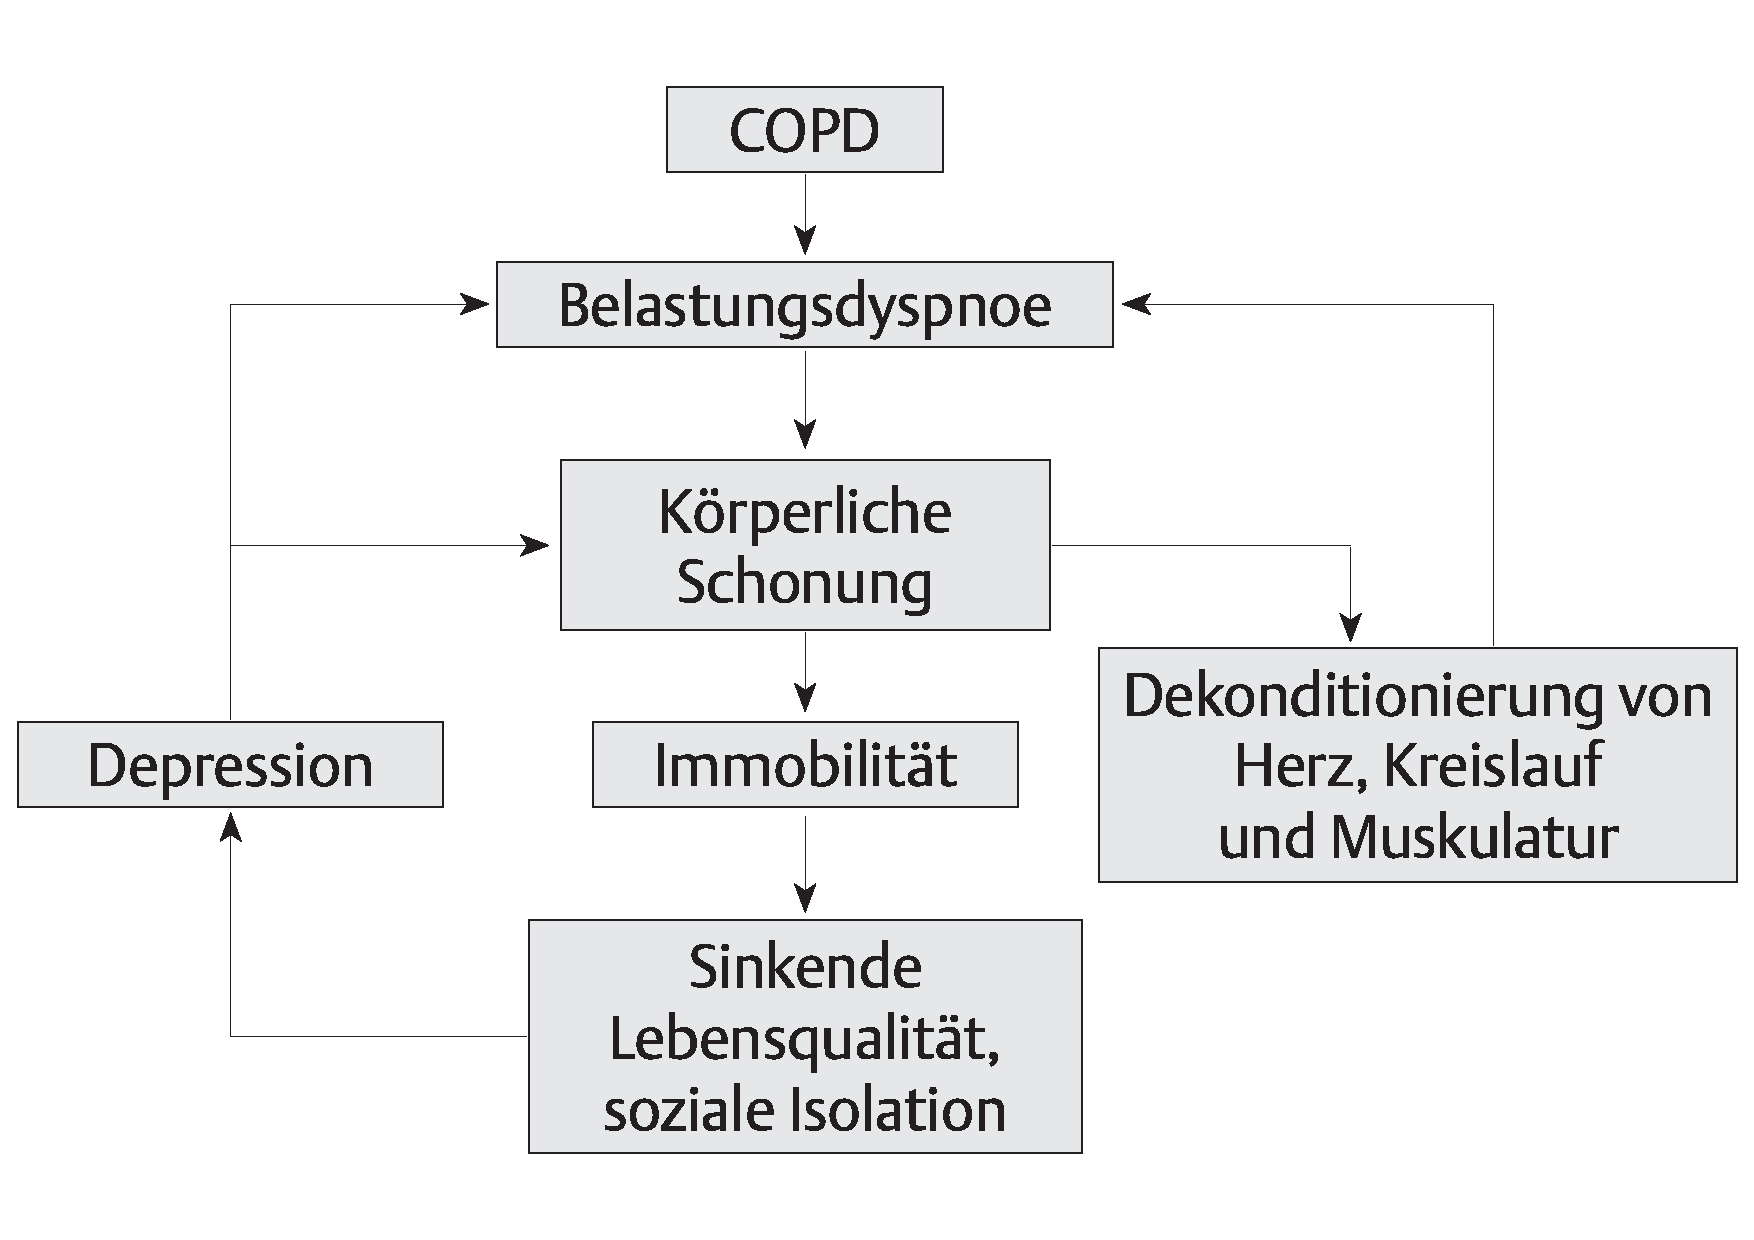
\includegraphics[width=0.6\textwidth]{teufelskreis}
  \caption{Circulus virtuosus, übernommen aus \cite[e19]{vogelmeier2007}}
  \label{fig:copd_teufelskreis}
\end{figure}

Die Angaben zur Prävalenz von Angst und Depression bei COPD variieren sehr. „Generalisierte Angststörungen werden in einer Häufigkeit von 2-16\%, Panikstörungen von 8-67\%, depressive Symptome und Depressionen zwischen 11 und 80\% sowie Angstsymptome in einem Bereich von 10-75\% angegeben“  \autocite[34]{kenn2011}.

An diesen Zahlen lässt sich erkennen, dass exakte Ergebnisse in Bezug auf die Prävalenz noch fehlen. Kenn und Kühl gehen davon aus, dass hierfür verschiedene methodische Diagnoseansätze verantwortlich sind. Generell erschwerte wohl neben den unterschiedlichen Erhebungsinstrumenten, wie Interviews und Fragebögen, auch die Heterogenität der untersuchten Patientenkohorte mit verschiedenen Schweregraden die Interpretation der Ergebnisse \autocite[vgl.][35]{kenn2011}.
Zudem geben die Studienergebnisse keine Auskunft darüber, in wieweit bei Patienten, die eine COPD aufgrund eines längeren Nikotinabusus entwickelt haben, bereits eine größere psychische Vulnerabilität und somit ein erhöhtes Risiko für die Ausbildung einer Depression oder Angst-/Panikstörung besteht. 

Ein evtl. wichtiges Konzept für den Krankheitsverlauf der COPD in seinen unterschiedlichen Facetten scheint die so genannten "`Fear Avoidance"' zu sein. Viele Patienten berichten von Angst vor auftretender Atemnot. Fear Avoidance- Konzept meint "`die Angst vor der Verstärkung eines Krankheitssymptoms bzw. Verschlechterung des Verlaufs und daraus folgende Aktivitätsvermeidung"' \autocite[111]{stenzel2013}. Dieses Konzept wurde jedoch bisher für COPD noch kaum diskutiert und erforscht. Eine neuere Studie zeigte jedoch, dass Fear Avoidance tatsächlich als Mediator des Zusammenhangs zwischen COPD-Status und Lebensqualität bzw. Gesundheitsstatus gesehen werden kann. Die Autoren plädieren daher dafür, dass im Rahmen der pneumologischen Rehabilitation auch psychotherapeutische Interventionen implementiert werden sollten, welche diesen Aspekt aufgreifen \autocite[vgl.][112]{stenzel2013}. 

In dem später dargestellten musiktherapeutischen Konzept wird dieser Aspekt ebenfalls implizit aufgenommen. Durch achtsames Wahrnehmen eigener Grenzen und Mög"-lichkeiten, aber auch übungszentriertes Arbeiten entwickeln die Patienten mithilfe positiver Erfahrungen im Zusammenhang mit Selbstregulation wieder mehr Selbstvertrauen und erleben sich als selbstwirksame Individuen, die sich nicht der auftretenden Atemnot ausgeliefert fühlen müssen.

In Studien wurde zudem ein signifikanter Zusammenhang zwischen einer erhöhten Mortalität und einer COPD mit begleitender depressiver oder Angstsymptomatik nachgewiesen. Aber auch in Bezug auf die Exazerbations- und Rehospitalisationsrate sowie die Leistungsfähigkeit und -bereitschaft von COPD-Patienten scheint hier die Ausbildung der genannten psychischen Erkrankung einen relevanten negativen Faktor darzustellen \autocite[vgl.][]{kenn2011}.

Obgleich das zuvor Erläuterte heutzutage unter allgemeinmedizinischen und pneumologischen Fachärzten als bekannt anzunehmen ist, wird die Problematik in den Arzt-Patienten-Gesprächen oftmals nicht thematisiert. Eine amerikanische Studie zeigte diese Diskrepanz zwischen der Prävalenz und Behandlungshäufigkeit psychischer Erkrankungen bei gleichzeitiger COPD. In einer Telefonumfrage von 1334 Patienten lagen bei 61\% psychische Auffälligkeiten, insbesondere Angstsymptome, vor. Lediglich 31\% dieser Patienten wurden diesbezüglich behandelt \autocite[vgl.][156]{fischer2007}.


\section{Zusammenfassende Betrachtung}
\label{zusammenfassende betrachtung}
Die vorherigen Ausführungen machen deutlich, um welch komplexes und schwerwiegendes Krankheitsbild es sich bei der COPD handelt. 
Durch Gespräche mit praktizierenden Lungenfachärzten und Betroffenen sowie durch Aussagen in unterschiedlichen Fachartikeln zeichnete sich für mich der Bedarf an psychologischer respensive psychotherapeutischer Begleitung sehr stark ab. Selbst in der pneumologischen Rehabilitation stellen Gespräche mit einem Psychologen ein freiwilliges Angebot dar. Aufgrund der meist starken Unterbesetzung an psychosozialem Fachpersonal ist die Versorgung hier meines Erachtens nur mangelhaft gegeben. Patienten, die sich eher in sich zurückziehen und wenig Eigeninitiative zeigen, haben so vermutlich nur geringe Chancen, eine Begleitung ihrer Bedürfnisse entsprechend zu erhalten. An dieser Stelle soll wie unter Kapitel \ref{section:gedanken_zum_setting} das in dieser Arbeit entwickelte musiktherapeutische Konzept greifen. Bevor jedoch auf dieses näher eingegangen wird, gibt das nächste Kapitel einen umfangreichen Einblick in das Thema "`Musiktherapeutische Stimmarbeit"' als solche.

% ---------------------------------------------------------------------------
% ----------------------- end of thesis sub-document ------------------------
\newpage\thispagestyle{empty}
% this file is called up by thesis.tex
% content in this file will be fed into the main document

%: ----------------------- introduction file header -----------------------
\chapter{Musiktherapeutische Stimmarbeit}
\label{chapter:musiktherapeutische_stimmarbeit}
\setlength{\epigraphwidth}{8.0cm}
\epigraph{Success depends upon previous preparation, and without such preparation there is sure to be failure.}{Confucius}
\ifpdf
    \graphicspath{{3_musiktherapeutische_stimmarbeit/figures/PNG/}{3_musiktherapeutische_stimmarbeit/figures/PDF/}{3_musiktherapeutische_stimmarbeit/figures/}}
\else
    \graphicspath{{3_musiktherapeutische_stimmarbeit/figures/EPS/}{3_musiktherapeutische_stimmarbeit/figures/}}
\fi
% ----------------------------------------------------------------------
%: ----------------------- introduction content -----------------------
% ----------------------------------------------------------------------
\lettrine{I}{n} this chapter, we introduce 


Herr \autocite[vgl.][12]{wolf2012} sagt, singen ist schön \autocite[9]{wolf2012}.
...them with 10Hz GNSS PVT\footnote{position, velocity, time} solutions. Because the MEMS-grade IMU exhibits a drift of more tha


\section{Einsatz der Singstimme in der Musiktherapie}
Bevor auf das Singen in der MT im Speziellen eingegangen wird, sollte der Blick auf den Gebrauch der Singstimme in der Gesellschaft gewendet werden, um ein klareres Gesamtbild dieses Themas entstehen lassen zu können.

Während das Singen, man beachte unseren großen Umfang an deutschem Liedgut, in unserer Großelterngeneration noch weit verbreitet war, so hat die nationalsozialistisch geprägte Zeit der 30er und 40er Jahre einen Keil in diesen selbstverständlichen Gebrauch der Singstimme in Gemeinschaft getrieben.
Die Verschandelung deutschen Liedguts mit nationalsozialistischem Gedankengut und den Einsatz desgleichen für propagandistische Zwecke sowie im Besonderen in der Jugendmusikbewegung der damaligen Zeit führte u.a. zu "der späteren Voreingenommenheit gegenüber gemeinsamem Singen im Allgemeinen und gegenüber dem deutschen Volkslied im Speziellen" \autocite[9]{wolf2012}.

Hinzu kommt die Entwicklung neuer Medien und die Möglichkeit eines geöffneten Zugangs zu diesen. Laut Wolf hat dies großen Einfluss auf "die Entwicklung hin zu einer Vereinzelung der Menschen und hin zu einer Veränderung des menschlichen Alltagverhaltens" \autocite[10]{wolf2012}, wodurch die Notwendigkeit der gemeinschaftlichen Freizeitgestaltung, welche in früheren Zeiten oftmals das gemeinsame Singen beinhaltete, nachließ. Nur an vereinzelten Schauplätzen wie z.B. im Gottesdienst, im Stadion, bei den Pfadfindern oder in Chören wird das gemeinschaftliche Singen und/oder Grölen noch aktiv praktiziert.

In der MT war der Einsatz der Singstimme ebenfalls lange Zeit negativ konnotiert und wurde "[\ldots] als "Konflikt vermeidende Technik" in den heilpädagogisch orientierten Bereich der Kindermusiktherapie oder das palliativ orientierte Feld der Geriatrie verortet" \autocite[10]{wolf2012}. So war das Singen von Liedern im Rahmen einer "psychotherapeutisch orientierten MT" lange Zeit ausgeklammert. Zudem wurde die Stimme zum klanglichen Ausdruck kaum genutzt, da man einen zu großen Widerstand seitens der Patienten erwartete. 

%Todo: Widerstand und Stimmeinsatz

Durch den sich in den letzten Jahren vollziehenden Paradigmenwechsel in der psychotherapeutischen Behandlung im Allgemeinen und der musiktherapeutischen im Speziellen von einem eher konfliktzentrierten Ansatz und dem Konzept der Katharsis hin zu einem eher ressourcenorientierten und stabilisierenden Arbeiten veränderte sich auch die Einstellung gegenüber dem Singen. Einer kleinen Forschergruppe aus Musiktherapeuten und -pädagogen, aber auch bekannten Ärzten (wie z.B. Dr. Gerald Hüther, Dr. Manfred Spitzer u.a.) ist es zu verdanken, dass wir heute mehr über die Wirkung des Singens auf Körper, Geist und Seele wissen. Sie waren es, die zu einer Etablierung von Singgruppenarbeit primär beigetragen haben. Im klinischen Bereich hat sich insbesondere Wolfgang Bossinger verdient gemacht und eine mittlerweile über Deutschland verbreitete Initiative, "Singende Krankenhäuser", ins Leben gerufen. Aber auch Sabine Rittner und Karl Adamek haben zu einem großen Erkenntnisgewinn und möglichen Vorgehensweisen in diesem Bereich verholfen.

Heute wird die (Sing-)Stimme im psychotherapeutischen Kontext in unterschiedlicher Art und Weise eingesetzt, genutzt und betrachtet. Sabine Rittner todo hat diese Bereiche kategorisiert, um ihre Komplexität zu entzerren. Diese insgesamt acht Kategorien fließen in die folgenden Ausführungen ein: 
Stimme als\ldots
\begin{enumerate}
\item Medium der verbalen und nonverbalen Beziehungsgestaltung
\item Methode in der körperorientierten Musikpsychotherapie
\item Diagnostikum im therapeutischen Gespräch
\item Indikator für die therapeutische Übertragung- und Gegenübertragung
\item Symptom
\item Ausdrucksmittel
\item Selbstheilungs-Mittel
\item Medium zur Tranceinduktion
\end{enumerate}
Im Rahmen der Diagnostik gibt die Stimme des Patienten bereits wichtige Hinweise auf dessen aktuelle Befindlichkeit, seine Stimmung und durch aufmerksames Hinhören kann erspürt werden, ob das Gesagte in sich "stimmig", sprich kongruent ist. Zudem gibt sie bereits Auskunft über den biografischen Hintergrund der sich äußernden Person, denn sie hat sich mit unseren über die Zeit gesammelten Lebenserfahrungen weiterentwickelt und diese in sich aufgesogen. So gilt die Stimme unter Experten als "Klingendes Hologramm der Persönlichkeit" \autocite{adamek1999} "lauthafte Biographie" \autocite{gundermann1994} und bei Rittner erfahren wir über den Klang der Stimme etwas über die "leib-seelische Gewordenheit" \autocite[211]{rittner2008} des Menschen.
Dabei scheint jedoch nicht so sehr der Inhalt des Gesagten aufschlussreich, sondern vielmehr der "Klang der Stimme (Klangspektrum, Modulation, Lautstärkeänderungen, Stimmsitz, Vokaleinsatz etc.), die Sprechweise (Artikulation, Phrasierung, Pausensetzung etc.) und die Atmung (Atemfrequenz, Atemtiefe, hörbares Einatmen, Sitz des Atemraumes im Körper etc.)" als auch "die Art der Gestaltung von Sprechpausen, Abbrüchen, Momenten des Innehaltens, Verzögerungen u.ä." \autocite[210]{rittner2008}. Diese stillen Momente, wie


Die Wirkung des Singens auf Körper und Psyche
Bossinger, Adamek und Cramer

Wirkungsfähigkeiten des Singens im therapeutischen Kontext

Die Rolle der Stimme für die Diagnostik




\newpage\thispagestyle{empty}
% ----------------------------------------------------------------------
\chapter{Andere wichtige therapeutische Ansaetze für die Arbeit mit COPD Patienten}
\label{chapter:andere_wichtige_therapeutische_ansaetze_für_die_arbeit_mit_copd_patienten}
%put your favorite quote
\epigraph{Choose a job you love, and you will never have to work a day in your life.}{Confucius}

% the code below specifies where the figures are stored
\ifpdf
    \graphicspath{{4_segmentation/figures/PNG/}{4_andere_wichtige_therapeutische_ansaetze_für_die_arbeit_mit_copd_patienten/figures/PDF/}{4_andere_wichtige_therapeutische_ansaetze_für_die_arbeit_mit_copd_patienten/figures/}}
\else
    \graphicspath{{4_andere_wichtige_therapeutische_ansaetze_für_die_arbeit_mit_copd_patienten/figures/EPS/}{4_andere_wichtige_therapeutische_ansaetze_für_die_arbeit_mit_copd_patienten/figures/}}
\fi

\lettrine{T}{his} chapter 


georef!
% this file is called up by thesis.tex
% content in this file will be fed into the main document

%: ----------------------- name of chapter  -------------------------
\chapter{Konzept}
\label{chapter:konzept}
\setlength{\epigraphwidth}{7.0cm}
\epigraph{To study and not think is a waste. To think and not study is dangerous.}{Confucius}

\section{Gedanken zu COPD und Singen}
Wenngleich der Einsatz der (Sing-)Stimme insbesondere im Hinblick auf ein bewussteres und verlängertes (Aus-)Atmen m.E. in diesem Bereich sehr sinnvoll erscheint, so ist gleichzeitig auch Vorsicht geboten. In diesem Bereich kann es zu entzündlichen Vorgängen rund um den Stimmapparat aufgrund der medikamentösen Behandlung und einer geschwächten Immunabwehr kommen. In diesen Fällen ist es notwendig, durch einen Phoniater abklären zu lassen, ob die Stimme der Schonung bedarf oder aber der gezielte und bedachte Einsatz der Stimme zu einer Besserung der Stimmfähigkeit beiträgt \autocite[vgl.][103ff.]{alavi2009}.
%: ----------------------- paths to graphics ------------------------
% change according to folder and file names
\ifpdf
    \graphicspath{{5_konzept/figures/PNG/}{5_konzept/figures/PDF/}{5_konzept/figures/}}
\else
    \graphicspath{{5_konzept/figures/EPS/}{5_konzept/figures/}}
\fi

\lettrine{T}{he} algorithm for

\newpage\thispagestyle{empty}
% ---------------------------------------------------------------------------
%: ----------------------- end of thesis sub-document ------------------------
% ---------------------------------------------------------------------------
%% this file is called up by thesis.tex
% content in this file will be fed into the main document

%: ----------------------- name of chapter  -------------------------
\chapter{Auswertung eigener Erfahrungen und Aufzeichnungen aus der Umsetzungsphase}
\label{chapter:auswertung_eigener_erfahrungen_und_aufzeichnungen_aus_der_umsetzungsphase}
\setlength{\epigraphwidth}{7.0cm}
\epigraph{By three methods we may learn wisdom: First, by reflection, which is noblest; second, by imitation, which is easiest; and third by experience, which is the bitterest.}{Confucius}

% change according to folder and file names
\ifpdf
    \graphicspath{{6_auswertung_eigener_erfahrungen_und_aufzeichnungen_aus_der_umsetzungsphase/figures/PNG/}{6_auswertung_eigener_erfahrungen_und_aufzeichnungen_aus_der_umsetzungsphase/figures/PDF/}{6_auswertung_eigener_erfahrungen_und_aufzeichnungen_aus_der_umsetzungsphase/figures/}}
\else
    \graphicspath{{6_auswertung_eigener_erfahrungen_und_aufzeichnungen_aus_der_umsetzungsphase/figures/EPS/}{6_auswertung_eigener_erfahrungen_und_aufzeichnungen_aus_der_umsetzungsphase/figures/}}
\fi

\lettrine{A}{s} input, the path planner requires the UAV's current position, the sparse collider cloud and a list of waypoints.



\chapter{Motion Control for Autonomous Flight}
\label{section_motion_control_for_autonomous_flight}

Multirotor UAVs require 

\newpage\thispagestyle{empty}
% ---------------------------------------------------------------------------
%: ----------------------- end of thesis sub-document ------------------------
% ---------------------------------------------------------------------------
%\chapter{Schlussbetrachtung und Ausblick} % top level followed by section, subsection
Für die erläuterten konzeptionellen Überlegungen im vorherigen Kapitel war es wichtig, sich im Vorherein ausgiebig mit den Themen COPD und musiktherapeutische Stimmarbeit auseinanderzusetzen, um ein grundlegendes Verständnis und Wissen für beide Bereiche entwickeln zu können. So wurde beispielsweise erst im Verlauf der Bearbeitung dieser Masterthesis immer deutlicher, dass der Suchtaspekt in den konzeptionellen Überlegungen aufgegriffen und mitgedacht werden muss. Inwieweit nun aber die bereits bestehende Suchtstruktur ursächlich mit der Ausbildung einer Depression oder Angststörung zusammenhängt oder aber tatsächlich die COPD-Erkrankung erst zu dieser Entwicklung führt, kann hier nicht beantwortet werden, stellt jedoch m.E. ein sehr interessantes Forschungsfeld dar. In Zusammenhang mit einer eventuell bestehenden Ich-Schwäche, wie sie im Suchtkontext vermutet wird, stellt das Medium "`Stimme"' meiner Meinung nach eine gute Möglichkeit dar, diesen Bereich zu stärken. Durch die Arbeit mit der Stimme kommen wir direkt in Kontakt mit unserem eigenen Gefühlsleben und unserer Körperwahrnehmung, so dass wir über das In-uns-hinein-spüren und -hören einen besseren Zugang zu diesen erreichen können. Über diese sensibilisierte Wahrnehmung wird es immer leichter, eigene Bedürfnisse zu erkennen und in einem nächsten Schritt sich für diese einzusetzen. Wie es sich anfühlt, eigenen Impulsen, Wünschen und Gefühlen zu folgen, kann in diesem geschützten therapeutischen Rahmen im Sinne eines Probehandelns ausgetestet werden. Durch das unmittelbar Körperliche in diesem musikalischen Handeln können die neuen Erfahrungen sowohl körperlich verankert als auch durch die anschließende verbale Reflexion kognitiv als Handlungsalternativen integriert werden.

Die Idee des Einsatzes musiktherapeutischer Stimmarbeit als Begleitbehandlung bei einer COPD-Erkrankung beruht auf der Überlegung, sich die ganzheitliche Wirkung der Stimmarbeit auf körperlicher und psychischer Ebene auch in diesem Bereich nutzbar zu machen (siehe u.a. Kapitel \ref{wirkung_des_singens}). Gerade in Bezug auf ein gestörtes "`Körperselbst"', wie es weiter oben bereits im COPD-Kontext erläutert wurde, könnte die Form der musiktherapeutischen Arbeit einen positiven Einfluss auf und Veränderungen für dieses bedeuten: Im stimmlichen Ausdruck liegt die Chance, sich selbst als Ganzes zu erleben und wahrzunehmen sowie einen positiven Körperbezug zu stärken. Darüber hinaus ist die Stärkung der Selbstwirksamkeit und des eigenen gesundheitsorientierten Handelns ein wesentlicher Gesichtspunkt für eine verbesserte Lebensqualität und Gesundheitszustand COPD-Betroffener. Dies kann m.E. jedoch nur gelingen, wenn die Gefühle der Ohnmacht und des Ausgeliefertseins (siehe Kapitel \ref{psychodynamische_ueberlegungen}) überwunden werden können und so das eigene Gestalten wieder möglich wird. Mit Hilfe des Stimmausdrucks ist es in besonderer, körpernaher Weise möglich, sich selbst sowie das eigene körperliche und seelische Befinden zu beeinflussen. 

Auch die soziale Funktion des Singens scheint mir im therapeutischen Kontext mit COPD-Betroffenen ein wichtiger Aspekt hinsichtlich der belegten Tendenz zu sozialer Isolation zu sein, denn mittels der "Brückenfunktion der menschlichen Stimme zwischen "`Innen"' (...) und "`Außen"' \autocite[283]{deckervoigt2000} können Teilnehmer sich im Kontakt mit anderen erleben und so ihr "`soziales Selbst"' stärken. Dieser Aspekt hat nicht nur Einfluss auf die psychische Verfassung, die Lebensqualität und das Wohlbefinden Betroffener, sondern auch auf die Mortalität. Wie eine Studie englischer Forscher um Andrew Steptoe im vergangenen Jahr zeigte, erhöht "`soziale Isolation"' die Mortalität \autocite[vgl.][]{pmid23530191}. So ist die Reduzierung sozialer Isolation zudem wichtig im Hinblick die Senkung des vorzeitigen Todesrisikos.

%Die Wirksamkeitsüberprüfung könnte sich jedoch als schwierig herausstellen, da die Patienten natürlich nicht von anderen wichtigen Therapien, wie z.B. Atemtherapie, ausgeschlossen werden können und somit . Es könnte jedoch über einen längeren Zeitraum 
%Schwierigkeit: unterschiedliche Schweregrade, Hintergründe, Erfahrungen mit dem Singen... es müssten also recht viele Daten erhoben werden. In einem ersten Schritt könnten jedoch sowohl an Teilnehmer dieses Gruppenangebots als auch an nicht teilnehmende, jedoch ebenfalls die pneumologische Rehabilitation in Anspruch nehmende Patienten Fragebögen ausgegeben werden, welche sich dem Thema "`Lebensqualität"' und "`Selbstwirksamkeit"' zuwenden, um einen Teil der Zielsetzungen bereits zu überprüfen. Hierfür gibt es bereits standardisierte Fragebögen, wie sie beispielsweise von Gunter Kreutz und Steven Clift in den zuvor genannten Studien eingesetzt wurden.

Wie bereits zuvor anklang, bestünde nun der nächste Schritt in der praktischen Umsetzung dieses Konzepts. Hierfür würde sich m.E. im Hamburger Raum besonders die "`Atem-Reha"' am Berliner Tor anbieten, da hier das Setting der oben mehrfach beschriebenen pneumologischen Rehabilitation gegeben ist. So können bereits die praktischen Erfahrungen zu einer Weiterentwicklung des Konzepts führen. Darüber hinaus bedarf es hierfür der weiteren Diskussion und des Erfahrungsaustauschs mit Kollegen, die ebenfalls in diesem Umfeld tätig sind, sowie schließlich der wissenschaftlichen Überprüfung des Konzepts in der Praxis hinsichtlich der beschriebenen Zielsetzungen. Wie auch Clift et al. (siehe Kapitel \ref{copd_in_der_singforschung}) denke ich, dass in einem ersten Schritt überhaupt getestet werden sollte, ob eine größere Untersuchung hinsichtlich der erzielten Effekte überhaupt sinnvoll erscheint. Für die Überprüfung der Teilziele "`Steigerung der Lebensqualität und Selbstwirksamkeit"' könnten bereits entwickelte, standardisierte Fragebögen eingesetzt werden, welche schon von Clift et al. und Kreutz eingesetzt wurden.

Kurz vor Abgabe dieser Arbeit wurde ich in meinem Ansinnen, ein musiktherapeutisches Konzept für die Arbeit mit COPD-Patienten zu entwickeln, sehr gestärkt. Das Beth-Israel-Hospital in New York, welches derzeit mit zu den führenden Forschungsinstituten für Musikmedizin und Musiktherapie zählt, stellt seit Ende Mai 2014 eine Teilnehmerkohorte für die Durchführung einer Studie zur Abklärung der Effekte auf die physische Funktionalität und Lebensqualität von Erwachsenen mit COPD mithilfe von Musiktherapie zusammen ("`The Effects of Music Therapy in the Treatment of Chronic Obstructive Pulmonary Disease"'). Dies zeigt meines Erachtens die Aktualität dieses Themas und lässt hoffen, dass Musiktherapie evtl. in naher Zukunft in die Standardtherapie bei COPD integriert wird. Abgesehen davon bleibt zu hoffen, dass sich die Situation hinsichtlich der psychosozialen Begleitung und Beratung von COPD-Betroffenen in den nächsten Jahren verbessert und sie frühzeitig eine ihren Bedürfnissen entsprechende Unterstützung erhalten.

Die Auseinandersetzung mit dem Thema "`Musiktherapeutische Stimmarbeit"' als solcher hat mir einmal mehr das Potenzial aufgezeigt, welches in der bewussten und achtsamen Auseinandersetzung mit unserem Körper, Atmung und Stimme liegt.
Diese Aspekte sollten m.E. auch in der musiktherapeutischen Arbeit mitgedacht und eingebettet werden. Um jedoch Patienten diesen Erfahrungsbereich eröffnen zu können, bedarf es zuvor der intensiven Beschäftigung mit der eigenen Stimme. Denn erst, wenn ich selbst gelernt habe, meine Stimme in mir frei und angenehm schwingen zu lassen, kann mich der Stimme anderer zuwenden \autocite[vgl.][15]{mcmurtry2012}. 
Dies hängt unter anderem mit dem in Kapitel \ref{scham_und_stimme} beschriebenen Resonanzphänomen, der klanglich-organismischen-Resonanz, zusammen: nur über die ausgiebige Auseinandersetzung mit und das Erleben der eigenen Stimme können Anspannungen oder Besonderheiten in der Stimme des Klienten wahrgenommen und nachvollzogen werden, wenn sie von der eigenen "`stimmlichen Verfassung"' abweichen. 
So können auf diesem Wege "`in seinem Stimmklang eine Enge oder Verspannung, Energielosigkeit, Druck oder Unbewusstheit in bestimmten Körperzonen" \autocite[16]{mcmurtry2012} entdeckt werden. 
Ein entspannter, selbstverständlicher und freier Umgang mit der eigenen Stimme erleichtert es unseren Klienten zudem, auch ihre Stimme als ganz individuelles Ausdrucksmittel zu nutzen.

Aus den hier zusammen getragenen Gründen erscheint mir die Einbettung dieses Themas in musiktherapeutische Theorie und Forschung als auch in die musiktherapeutische Ausbildung als sehr wichtig. Die Entwicklungen der letzten Jahre geben Grund zur Hoffnung, dass sich das Singen sowohl als musiktherapeutische Methode als auch gesamt-gesellschaftlich wieder mehr etabliert.


\newpage\thispagestyle{empty}
% ---------------------------------------------------------------------------
%: ----------------------- end of thesis sub-document ------------------------
% ---------------------------------------------------------------------------



% --------------------------------------------------------------
%:                  BACK MATTER: appendices, refs,..
% --------------------------------------------------------------

% the back matter: appendix and references close the thesis
% this file is called up by thesis.tex
% content in this file will be fed into the main document

%: ----------------------- name of chapter  -------------------------
%\appendix
\phantomsection
\renewcommand{\chaptername}{Anhang} % uncomment to print only "1" not "Chapter 1"
\renewcommand\thechapter{\Alph{chapter}}
\setcounter{chapter}{0}
%\appendix
\chapter{} % top level followed by section, subsection
\label{chapter:appendix}


%: ----------------------- paths to graphics ------------------------

% change according to folder and file names
\ifpdf
    \graphicspath{{X/figures/PNG/}{X/figures/PDF/}{X/figures/}}
\else
    \graphicspath{{X/figures/EPS/}{X/figures/}}
\fi

%: ----------------------- contents from here ------------------------
%\begin{sloppypar}
%\lettrine{T}{he} source code for all proposed algorithms in this dissertation, including 
%end{sloppypar}



\newpage\thispagestyle{empty}









% ---------------------------------------------------------------------------
%: ----------------------- end of thesis sub-document ------------------------
% ---------------------------------------------------------------------------



%: ----------------------- bibliography ------------------------

% The section below defines how references are listed and formatted
% The default below is 2 columns, small font, complete author names.
% Entries are also linked back to the page number in the text and to external URL if provided in the BibTex file.

% PhDbiblio-url2 = names small caps, title bold & hyperlinked, link to page
%\begin{multicols}{2} % \begin{multicols}{ # columns}[ header text][ space]
%\begin{tiny} % tiny(5) < scriptsize(7) < footnotesize(8) < small (9)



\printbibliography[]
%\bibliographystyle{Latex/Classes/PhDbiblio-url2} % Title is link if provided
%\begin{footnotesize}
%\bibliographystyle{alpha}
%\bibliographystyle{natbib}
%\renewcommand{\bibname}{Referenzen} % changes the header; default: Bibliography
%\bibliography{bibliography} % adjust this to fit your BibTex file
%\end{footnotesize}
%\end{tiny}
%\end{multicols}
\newpage\thispagestyle{empty}
%\chapter*{Eidesstattliche Versicherung} 

Hiermit erkl\"are ich an Eides statt, dass ich die vorliegende Dissertationsschrift selbst
verfasst und keine anderen als die angegebenen Quellen und Hilfsmittel benutzt habe.

\vspace{150pt}
\noindent Hamburg, den \hfill Unterschrift

\vspace{30pt}
\noindent \rule{\textwidth}{0.5pt}

% --------------------------------------------------------------
% Various bibliography styles exit. Replace above style as desired.

% in-text refs: (1) (1; 2)
% ref list: alphabetical; author(s) in small caps; initials last name; page(s)
%\bibliographystyle{Latex/Classes/PhDbiblio-case} % title forced lower case
%\bibliographystyle{Latex/Classes/PhDbiblio-bold} % title as in bibtex but bold
%\bibliographystyle{Latex/Classes/PhDbiblio-url} % bold + www link if provided

%\bibliographystyle{Latex/Classes/jmb} % calls style file jmb.bst
% in-text refs: author (year) without brackets
% ref list: alphabetical; author(s) in normal font; last name, initials; page(s)

%\bibliographystyle{plainnat} % calls style file plainnat.bst
% in-text refs: author (year) without brackets
% (this works with package natbib)

%: Declaration of originality

% Thesis statement of originality -------------------------------------

% Depending on the regulations of your faculty you may need a declaration like the one below. This specific one is from the medical faculty of the university of Dresden.

\begin{declaration}        %this creates the heading for the declaration page

Hiermit versichere ich, dass ich die Arbeit selbständig verfasst und keine anderen als die angegebenen Quellen und Hilfsmittel benutzt habe.

\vspace{15mm}

Hamburg, 24. Juni 2014

\vspace{1,5 cm} 
\begin{tabular}{p{7cm}p{.5cm}l}
\hline \\ 
Sarah Fritzsche
\end{tabular}% 


\end{declaration}


% ----------------------------------------------------------------------

\end{document}
